\begin{defn}
	On dit qu'une partie $K \subset E$ d'un espace vectoriel normé (de dimension potentiellement infinie) $E$ est \textit{compacte} si, de toute suite $(\vec{u}_n)$ de vecteurs de $K$, on peut extraire une suite convergent vers un vecteur $\vec{\ell} \in K$, \textit{i.e.}, il existe une fonction $\varphi : \N\to \N$ strictement croissante telle que $\lim_{n\to \infty} \vec{u}_{\varphi(n)}$ existe et appartient à $K$.
\end{defn}

\begin{thm}[Bolzano-Weiersta\ss]
	De toute suite réelle bornée, on peut extraire une suite convergente (\textit{i.e.} tout segment de $\R$ est compacte).
	\qed
\end{thm}

\begin{rmk}
	Soit $(\vec{u}_n)_{n\in\N}$\/ une suite de vecteurs d'un espace vectoriel normé $E$.
	On dit qu'un vecteur $\vec{a} \in E$ est une \textit{valeur d'adhérence} de $(\vec{u}_n)_{n\in\N}$ si on peut extraire de $(\vec{u}_n)_{n\in\N}$ une suite convergent vers $\vec{a}$.
	\begin{enumerate}
		\item Par définition, une partie $K$ de $E$ est compacte si, et seulement si, toute suite de vecteurs possède au moins une valeur d'adhérence.
		\item La suite réelle définie par $u_n = n$ ne possède aucune valeur d'adhérence, et elle n'est pas bornée. 
		\item Une suite réelle, même bornée, peut posséder plusieurs valeurs d'adhérence.
			Par exemple, les valeurs d'adhérence de la suite de réels $(-1)^n$ sont $-1$ et $1$.
		\item Mais, si une suite de vecteurs est convergente, alors elle possède une unique valeur d'adhérence (égale à sa limite) : c'est la proposition 14 du chapitre 13.
			En contraposant, on a : si une suite possède plusieurs valeurs d'adhérence, alors elle diverge (on prouve ainsi que la suite des réels $(-1)^n$ diverge).
		\item La réciproque est fausse : la suite $(u_n)$ définie par $u_{2p} = =1$ et $u_{2p+1} = p$ possède une unique valeur d'adhérence (égale à $1$), mais elle diverge.
		\item Hormis dans un compact, où elle est vraie. $\triangleright$ Proposition suivante
	\end{enumerate}
\end{rmk}

\begin{prop}
	Une suite de vecteurs d'un compact $K$ converge si, et seulement si, elle possède une unique valeur d'adhérence.
\end{prop}

\begin{prv}
	\begin{itemize}
		\item[\guillemotleft~$\implies$~\guillemotright]
			Si une suite $(\vec{u}_n)_{n\in\N}$ converge vers une limite $\vec{\ell}$, alors toute suite extraite de $(\vec{u}_n)_{n \in \N}$ converge aussi vers $\vec{\ell}$.
			D'où, $\vec{\ell}$ est l'unique valeur d'adhérence de $(\vec{u}_n)_{n\in\N}$.
		\item[\guillemotleft~$\impliedby$~\guillemotright]
			On suppose que $(\vec{u})_{n \in \N}$ possède une unique valeur d'adhérence $\vec{\ell}$. Montrons, par l'absurde, que la suite $\vec{u}_n$ converge.
			Supposons donc que $(\vec{u}_n)_{n \in \N}$ ne converge pas vers $\vec{\ell}$.
			Autrement dit, il existe $\varepsilon > 0$ tel que, pour tout $N \in \N$, il existe $n \ge N$ tel que $\|\vec{u}_n - \vec{\ell}\| \ge \varepsilon$.
			On en déduit que l'on peut extraire de $(\vec{u}_n)_{n \in \N}$ une suite $(\vec{v}_n)_{n \in \N}$ qui ne rentre jamais dans la boule $\bar{B}(\vec{\ell},\varepsilon)$.
			Or, pour tout $n \in \N$, le vecteur $\vec{v}_{n}$ appartient à $K$, un compact.
			D'où, par définition, on peut extraire de la suite $(\vec{v}_n)_{n \in \N}$ une suite $(\vec{w}_n)_{n \in \N}$ qui converge vers $\vec{\ell}'$.
			Et, $(\vec{w}_n)_{n \in \N}$ est une suite extraite de $(\vec{u}_n)$.
			D'où, $\vec{\ell}'$ est une valeur d'adhérence de $(u_n)_{n\in\N}$. Or, $\vec{\ell} \neq \vec{\ell}'$, ce qui est absurde.
	\end{itemize}
\end{prv}

\begin{lem}
	\begin{enumerate}
		\item[(\textit{i})] Toute partie fermée d'un compact est un compact.
		\item[(\!\,\!(\textit{ii})\!\,\!)] Le produit cartésien de deux compacts est un compact. (Par récurrence pour un produit fini de compact)
	\end{enumerate}
\end{lem}

\begin{prv}
	\begin{enumerate}
		\item[(\textit{i})] On suppose $F \subset K$, où $F$ est un fermé et $K$ est un compact.
			Montrons que $F$ est compact.
			Soit $(\vec{u}_n)_{n\in\N}$ une suite de vecteurs de $F$ : $\forall n \in \N$, $\vec{u}_n \in F$.
			Or, $F \subset K$, d'où, $\forall n \in \N$, $\vec{u}_n \in K$.
			Et, $K$ est un compact, on peut donc extraire de $(\vec{u}_n)$ une suite $(\vec{v}_n)$ qui converge dans $K$.
			Soit ainsi $\vec{\ell} = \lim \vec{v}_n$.
			De plus, pour tout $n \in \N$, $\vec{v}_n \in F$ et $F$ est un fermé.
			D'où, $\vec{\ell} \in F$ par la caractérisation séquentielle d'un fermé.
		\item[(\!\,\!(\textit{ii})\!\,\!)]
			Soient $K_1$ et $K_2$ deux compacts.
			Montrons que $K_1 \times K_2$ est un compact.
			Soit $\big((\vec{u}_n, \vec{v}_n)\big)_{n \in \N}$ une suite d'éléments de $K_1 \times K_2$.
			Pour tout $n \in \N$, $\vec{u}_n \in K_1$, qui est un compact.
			On extrait donc de $(\vec{u}_n)$ une suite $(\vec{u}_{\varphi(n)})$ qui converge dans $K_1$.
			De la suite $(\vec{v}_{\varphi(n)}$, on extrait la suite $(\vec{v}_{\varphi(\psi(n))})$ qui converge dans $K_2$.
			La suite $\big((\vec{u}_{\varphi(\psi(n))}, \vec{v}_{\varphi(\psi(n))})\big)$ converge dans $K_1 \times K_2$ car $(\vec{u}_{\varphi(\psi(n))})$ converge dans $K_1$ et $\vec{v}_{\varphi(\psi(n))}$ converge dans $K_2$.
	\end{enumerate}
\end{prv}

\begin{prop}
	\begin{enumerate}[label=(\textit{\roman*})]
		\item Toute partie compacte d'un espace vectoriel normé est fermée et bornée.
		\item La réciproque est vraie dans $\R^n$ : une partie de $\R^n$ est fermée si, et seulement si, elle est fermée et bornée.
	\end{enumerate}
\end{prop}

\begin{exo}
	\begin{slshape}
		Montrer que
		\begin{enumerate}[label=(\textit{\alph*})]
			\item toute intersection de compacts est un compact ;
			\item l'union de deux compacts est un compact (de même, par récurrence, pour une union finie de compacts).
		\end{enumerate}
	\end{slshape}
\end{exo}

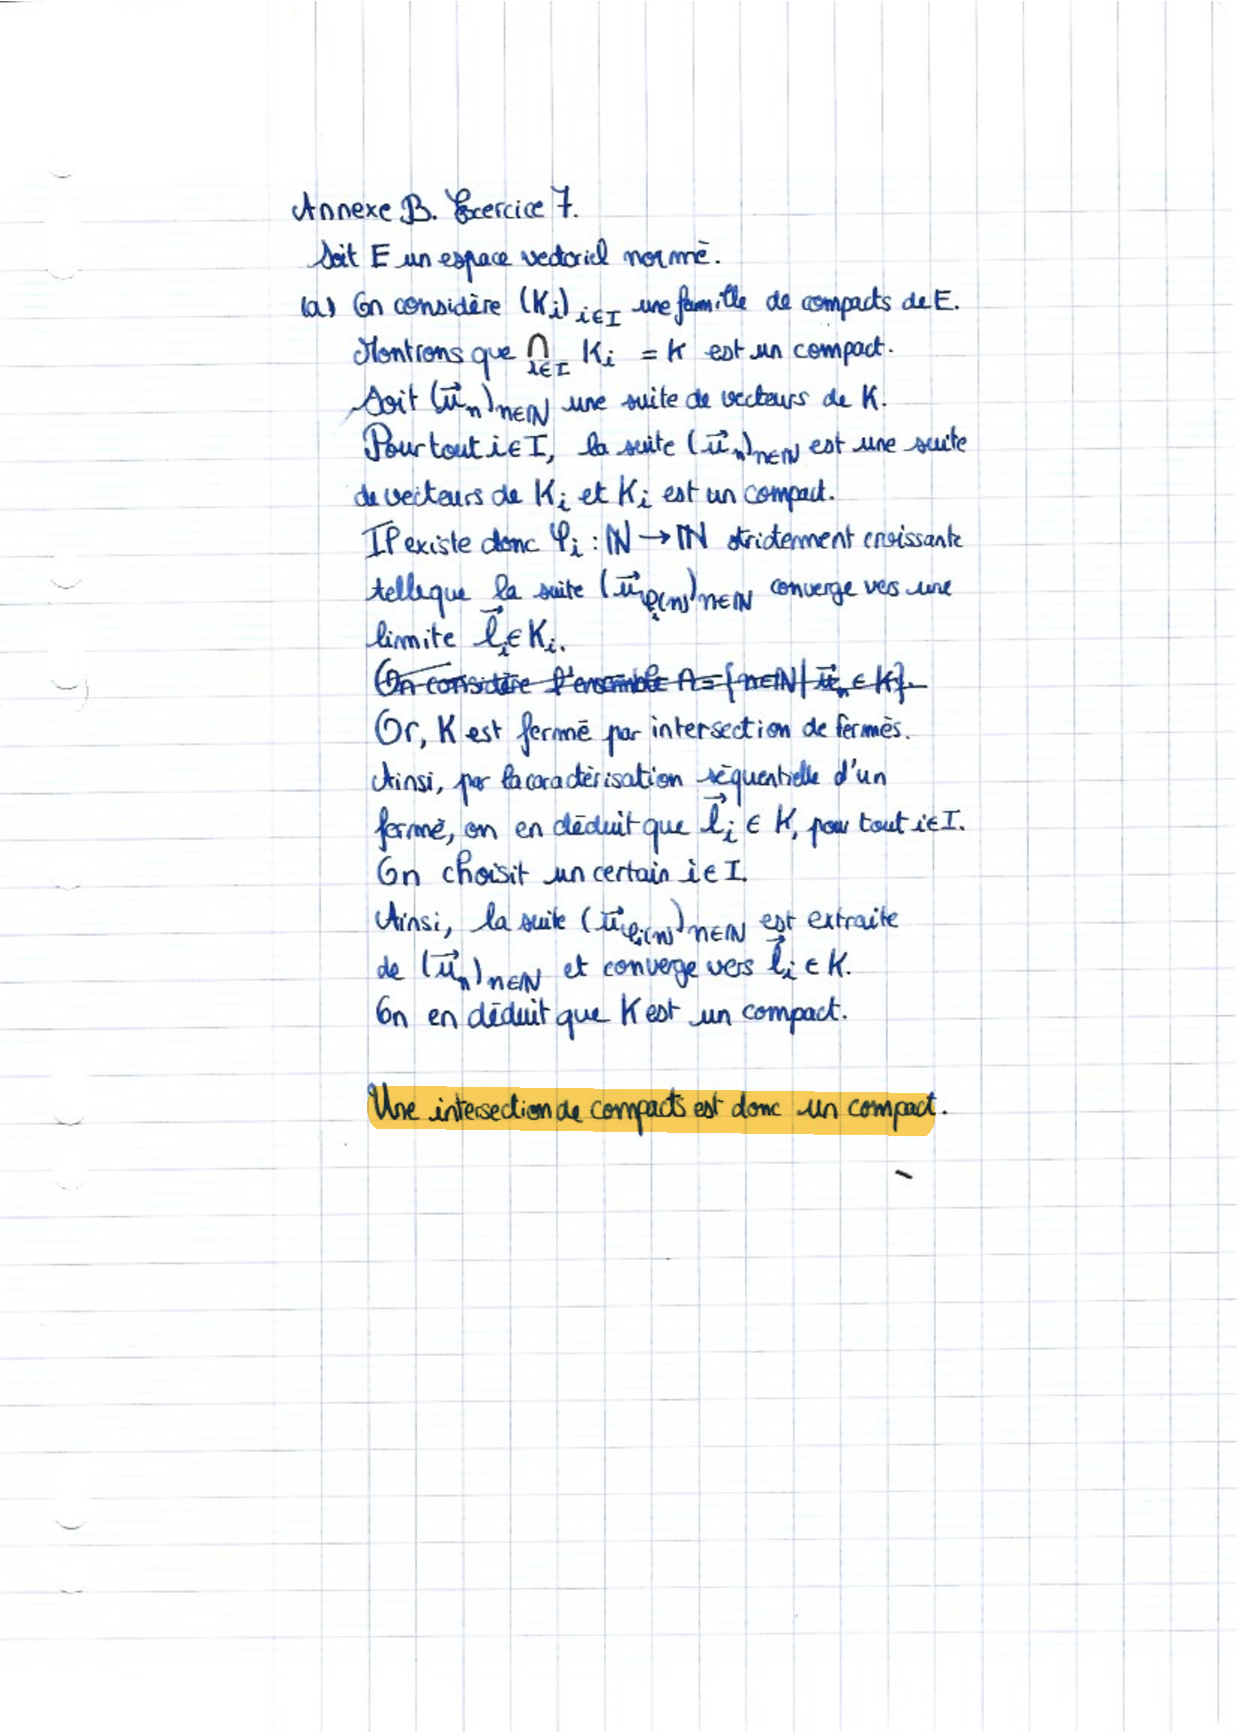
\includepdf[pages=-]{exo7.pdf}

\begin{prop}
	Soient $E$ et $F$ deux \textit{evn} de dimensions potentiellement infinies.
	Soit une fonction continue $f : E \to F$. Si $K \subset E$ est un compact de $E$, alors $f(K)$ est un compact de $F$.
	Autrement dit, \guillemotleft~l'image d'un compact par une fonction continue est un compact.~\guillemotright\@
	En particulier, toute fonction réelle continue sur un compact est bornée et atteint ses bornes.
\end{prop}

\begin{prv}
	Soit $(\vec{v}_n)$ une suite de vecteurs de $f(K)$.
	On veut extraire une suite de $f(K)$ qui converge dans $f(K)$.
	Pour tout $n \in \N$, il existe $\vec{u}_n \in K$ tel que $\vec{v}_n = f(\vec{u}_n)$.
	Or, $K$ est un compact.
	On peut donc extraire de $(\vec{u}_n)$ de vecteurs $(\vec{u}_{\varphi(n)})$ qui converge dans $K$, on note $\vec{\ell}$ sa limite.
	Ainsi, $\vec{u}_{\varphi(n)} \to \vec{\ell}$ et, comme $f$ est continue, $f(\vec{u}_{\varphi(n)}) \to f(\vec{\ell})$. D'où, $f(K)$ est un compact.
\end{prv}


\begin{prop}
	\ldots
\end{prop}

\begin{exo}
	\begin{slshape}
		On munit l'espace vectoriel $\R[X]$ de la norme définie par $\|P\| = \max_{k \in \llbracket 0,\deg P \rrbracket}\:|a_k|$\/ pour tout polynôme $P = \sum_{k=0}^{\deg P} a_k X^k$. Montrer que la partie $F = \{P \in \R[X]  \mid \|P\| = 1\}$ est une partie fermée et bornée de $\R[X]$, mais ce n'est pas un compact.
	\end{slshape}

	Afin de valider que $\|\cdot\|$ est une norme, on pose $\|0\| = 0$.
	La partie $F$ est la sphère centrée en $0$ et de rayon 1 : $\mathcal{S}(0, 1) = \bar{B}(0, 1) \setminus \mathring B(0, 1)$.
	Elle est donc bornée : $\forall P \in F$, $\|P\| = 1 \le 1$.
	De plus, $F$ est un fermé car $F = \|\cdot \|^{-1}(\{1\})$, $\|\cdot\|$ est continue (car toute norme est 1-lipschitzienne) et $\{1\}$ est un fermée.
	Mais, $F$ n'est pas un compact. En effet, on considère la suite de polynôme $(P_n)$ définie par $P_n = X^n$.
	Pour tout $n \in \N$, $\|P_n\| = \max(0,1) = 1$.
	Par l'absurde, supposons que l'on peut extraire de $(P_n)$ une suite $(X^{\varphi(n)})$ convergente, et on note $\ell$ sa limite.
	Or, $\|X^{\varphi(n)} - X^{\varphi(n +1)}\| = \max(-1, 0, 1) = 1$.
	Et, les égalités passent à la limite, $0 = \|\ell - \ell\| = 1$, ce qui est absurde.
\end{exo}

\begin{thm}[Heine]
	Toute fonction continue sur un compact est uniformément continue.
\end{thm}

